\documentclass[PhD-Yoann-Dupont.tex]{subfiles}
\begin{document}

Les réseaux de neurones (NN) sont des modèles inspirés du neurone formel défini par \citet{mcculloch1943logical}, illustré sur la figure \ref{fig:mcculloch-pitts-neuron}, ainsi que des théories connectionnistes décrites par \citet{hebb1949organisation}, dont le principe est souvent résumé à «\ les neurones qui s'activent en même temps, se lient entre eux\ », principe théorisant que, lorsqu'un cerveau reçoit un stimulus particulier ou effectue une tâche particulière, les neurones utilisés tendent à se regrouper entre eux. Dans le domaine des réseaux de neurones artificiels, cette théorie peut se reformuler en «\ les neurones s'activant en même temps représentent une même fonction\ ». En effet, la structure d'un réseau de neurones artificiel étant généralement fixe, seuls les différents poids reliant les différentes couches peuvent changer. Le réseau de neurones le plus simple est le perceptron \citep{rosenblatt1958perceptron}, qui suit exactement le modèle du neurone formel de la figure \ref{fig:mcculloch-pitts-neuron}, ce dernier est donc un réseau de neurones possedant un unique neurone, utilisé pour effectuer de la classification binaire. Ce dernier utilise la fonction de Heaviside, ou la fonction \emph{échelon-unité}\footnote{on la nomme plus couramment fonction \emph{step}.}, afin de produire sa sortie.

\begin{figure}[ht!]
\centering
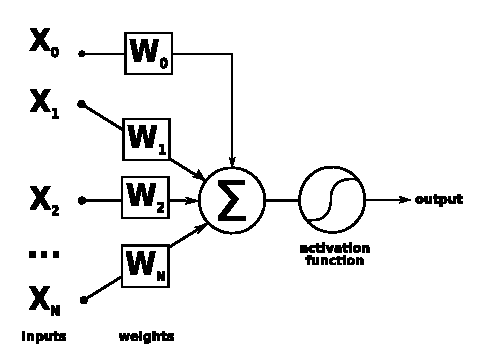
\includegraphics[scale=1.0]{images/NN/McCulloch-Pitts-neuron}
\caption{Une représentation schématique du neurone formel de McCulloch-Pitts. Il s'agit du modèle utilisé pour le perceptron.}
\label{fig:mcculloch-pitts-neuron}
\end{figure}

Le perceptron est un système dit monocouche, il modélise une unique fonction. Le perceptron multicouche, son évolution, représente la composition d'un ensemble de fonctions. D'un point de vue plus mathématique, les différentes couches [1, ..., N] d'un réseau de neurones représentent la composition d'un ensemble de fonctions [f$_{1}$, ..., f$_{N}$], écrite f$_{1}$ $\circ$ ... $\circ$ f$_{N}$. Si l'ensemble des fonctions f$^{N}_{i=1}$ étaient linéaires, alors leur composition serait également une fonction linéaire. Cela signifie qu'il existerait une fonction linéaire $g$ telle que $g$ = f$_{1}$ $\circ$ ... $\circ$ f$_{N}$. En conséquence, il serait possible de modéliser un perceptron multicouche à l'aide d'un perceptron monocouche, l'expressivité du modèle serait donc identique. Afin d'augmenter cette dernière, des fonctions non-linéaires, monotones, non-constantes, bornées et continues doivent être utilisées au sein du réseau multicouche, ce qui leur confère la capacité d'approximer n'importe quelle fonction continue selon le théorème d'approximation universelle \citet{cybenko1989approximation,hornik1991approximation}. Ces fonctions sont appelées, dans les réseaux de neurones, des \emph{fonctions d'activation} et ont généralement une forme sigmoïdale. L'une des premières fonctions d'activation est la sigmoïde :

\begin{equation}\label{eq:sigmoid}
\sigma(x) = \frac{1}{1 + e^{-x}} = \frac{e^{x}}{1 + e^{x}}
\end{equation}

Les réseaux de neurones comme le perceptron font partie de la famille des \emph{feedforward neural network} (FFNN) \citep{rosenblatt1958perceptron,svozil1997introduction}, où l'information dans ces réseaux ne circulent que dans un sens unique : vers l'avant. Ils peuvent se représenter par des graphes orientés acycliques.
L'inconvénient des FFNN est dans leur fonction de décision est intrinsèquement locale. En effet, si l'on traite des séquences comme illustré dans la section \ref{sec:machine-learning}, ces réseaux ne savent pas modéliser les dépendences qui peuvent exister au niveau de la séquence et sont donc sujets à des erreurs d'annotation comme celles de la figure \ref{tab:ner-tagging-example}.
Afin de modéliser ces dépendences typiques des données séquentielles les \emph{recurrent neural networks} (RNN) \citep{elman1990finding,mandic2001recurrent} ont été développés. Ces réseaux sont capables de faire transiter l'information à des couches précédentes, autrement dit en arrière. Ces réseaux ne peuvent pas être représentés par un graphe acylique. Une représentation simple de la différence entre un réseau de neurones classiques et un récurrent est donnée dans la figure\ \ref{fig:FFNN-vs-RNN}.

\begin{figure}[ht!]
\begin{minipage}{0.49\linewidth}
\centering
\includegraphics[scale=0.75]{images/NN/FFNN}
\end{minipage}
\begin{minipage}{0.49\linewidth}
\centering
\includegraphics[scale=0.75]{images/NN/Elman-RNN}
\end{minipage}
\caption{À gauche, un réseau de neurones classique. À droite, un réseau de neurones récurrent (Elman)}
\label{fig:FFNN-vs-RNN}
\end{figure}

\begin{figure}[ht!]
\centering
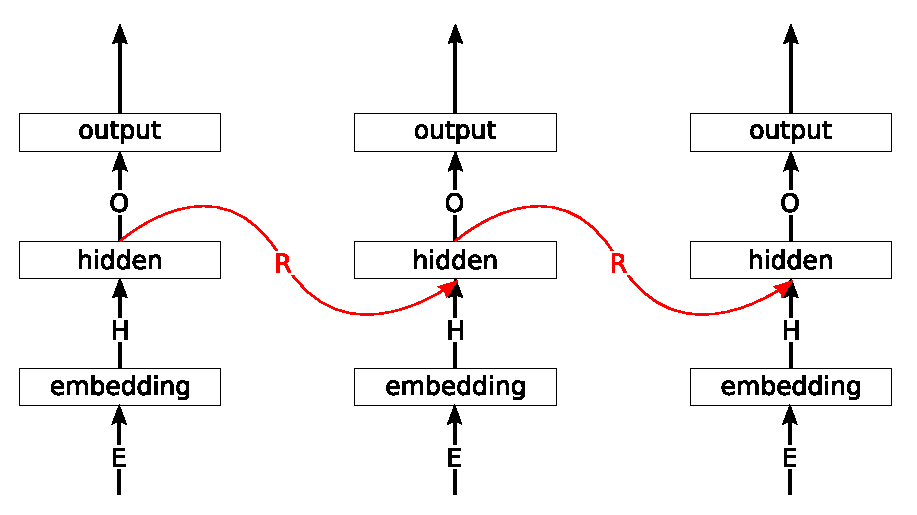
\includegraphics[scale=0.75]{images/NN/Elman-unrolled}
\caption{Un réseau d'Elman déroulé}
\label{fig:unrolled-RNN}
\end{figure}

À l'apprentissage, les paramètres $\theta$ du réseau de neurones sont, comme décrit précédemment pour les CRF, ajustés selon le maximum de log vraisemblance :

\begin{equation} \label{eq:NN-log-likelihood}
l(\theta) = \sum_{i=1}^{N} \log p(y^{i} | x^{i}, \theta)
\end{equation}

Où $x$ correspond à une observation (un token particulier dans une phrase, une phrase entière, etc... selon la tâche) et $y$ correspond à la sortie attendue. Quand l'ensemble de sortie $\mathcal{C}$ est discret et que chaque token est considéré indépendemment, la sortie du réseau $f_{\theta}(x)$ est un vecteur de taille $|\mathcal{C}|$ où chaque élément est le score associé à un élément de $\mathcal{C}$. Le score $f_{\theta}(x)_{i}$ d'un élément à l'indice $i$ peut s'interpréter comme sa probabilité conditionnelle $p(i|x,\theta)$ en lui appliquant une \emph{normalisation exponentielle}, appelée également \emph{softmax} :

\begin{equation} \label{eq:softmax}
softmax(x)_{i} = \frac{e^{x_{i}}}{\sum_{j=1}^{C}e^{x_{j}}}\ pour\ 1 \leq i \leq C
\end{equation}

L'apprentissage du modèle se fait de manière similaire aux CRF via une descente de gradient stochastique en minimisant une fonction objectif, traditionnellement la cross-entropie régularisée avec une norme $\ell^{2}$, qui se définit de la façon suivante :

\begin{equation} \label{eq:cross-entropy}
C = - c_{t} log( y_{t} ) + \frac{\lambda}{2} \left | \theta \right |^{2}
%\mathcal{C}(\theta) = - \frac{1}{n} \sum^{n}_{i=1} [y^{i}\log(h_{\theta}(x^{i})) + (1-y^{i})\log(1-h_{\theta}(x^{i}))]
\end{equation}

Où $\lambda$ est un hyper-paramètre, $c_{t}$ est une représentation dite "one-hot" de l'étiquette de référence. Cette représentation est l'équivalent d'un index dans un lexique : un vecteur "one-hot" est un vecteur où l'ensemble des valeurs est égale à 0, sauf à un unique indice, où la valeur est de 1.
%Où $\theta$ représente les paramètres du modèle, $n$ est le nombre d'exemples, ${y}^{i}$ la sortie attendue, $h_{\theta}(x^{i})$ la l'hypothèse prédite par le modèle pour l'entrée $x^{i}$.

La mise-à-jour des poids du modèle s'effectue à l'aide de la rétropropagation des erreurs \citep{linnainmaa1970representation,werbos1982applications,rumelhart1985learning}, qui consiste à évaluer la différence entre la sortie fournie par le modèle et la sortie attendue, avant de propager la différence à travers le réseau. Cet algorithme n'est pas directement appliquable sur un RNN en raison de sa nature récursive. Afin de mettre à jour les paramètres d'un RNN, une version adaptée de la rétropropagation a été créée : la rétropropagation à travers le temps \citep{werbos1990backpropagation}. Cet algorithme consiste à dérouler le RNN sur la séquence, comme illustré dans la figure\ \ref{fig:unrolled-RNN}, le réseau devient alors comparable à un FFNN, à la différence que certaines informations seront également envoyées à l'élément suivant dans la séquence. Un RNN a une structure comparable à une liste chaînée : chaque élément ne connait que son successeur direct, auquel il envoit sa sortie qui servira alors de contexte à ce dernier. Le côté récurrent du réseau s'obtient alors naturellement, l'information étant propagée de proche en proche, chaque élément de la séquence aura donc les contextes accumulés de tous ses prédécesseurs. Il est alors possible d'appliquer la rétropropagation classique sur le réseau déroulé.

Il ont récémment été repopularisé dans le TAL, notamment depuis l'avènement du deep learning \citep{hinton2007learning,bengio2015deep}, où les réseaux de neurones ont de nombreuses couches. Particulièrement, ils disposent de plusieurs couches utilisant des fonctions d'activation, alors que les réseaux n'en utilisaient qu'une. Un autre intérêt du deep learning est l'utilisation de représentations denses pour les tokens, que nous détaillerons dans la prochaine section.

\begin{comment}
avec \citet{collobert2008unified}.
Ils ont été récemment repopularisés dans le TAL avec les réseaux de neurones à convolution, ou CNN, \citep{collobert2008unified}, dont une illustration est disponible dans la figure\ \ref{fig:CNN-collobert2008} ainsi que. Actuellement, les réseaux les plus couramment utilisés sont de la famille des réseaux de neurones récurrents \citep{martens2011learning}. L'inconvénient de ces derniers est la difficulté de modéliser des dépendances longue distance ainsi que les problèmes d'extinction et d'explosion du gradient tels que décrits par \citet{bengio1994learning}. Pour compenser ce problème, le réseau LSTM \citep{hochreiter1997long,gers2000learning} a été proposé, permettant ainsi de conserver des dépendances longue distance. Bien que le réseau LSTM ait gagné en populatrité il y a peu, leur utilisation dans le domaine du TAL n'est pas si récente : l'une de leur première, si ce n'est la première, utilisation d'un tel réseau dans le TAL ayant été faite par \citet{hammerton2001clause,hammerton2003named} (défi CoNLL-2001 et données de CoNLL 2003, mais pas durant le défi). Le fonctionnement basique d'une cellule de LSTM (ou élément dans une séquence) est montré dans la figure \ref{fig:lstm-cell} On utilise aujourd'hui surtout le Bi-LSTM-CRF \citep{huang2015bidirectional} qui est de plus en plus populaire. Plus récemment, des modèles combinés de LSTM et CRF ont été utilisés \citep{lample2016neural}, un LSTM servant d'entrée à un CRF, pour obtenir des performances dans l'état de l'art actuel sur les différents corpus du CoNLL 2003. Le modèle cascade deux LSTM et un CRF. Le premier LSTM calcule une représentation des tokens à partir de ses caractères, ce qui permet de représenter sa morphologie. Cette représentation est ensuite concaténée à celle du second LSTM, qui calcule une représentation du token courant étant donné son contexte dans la phrase. Ce modèle permet donc d'avoir, pour chaque token, l'équivalent d'une analyse morphologique et d'un contexte syntaxique. La sortie de ce LSTM est alors donnée à un CRF, permettant d'établir des dépendances sur l'espace de sortie.

\begin{figure}[ht!]
\centering
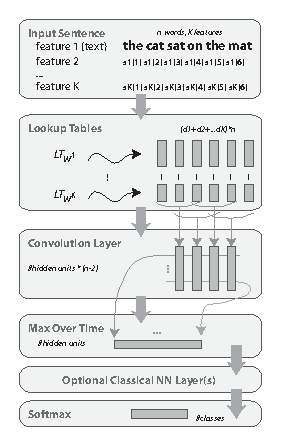
\includegraphics[scale=1.25]{images/general/collobert2008}
\caption{un réseau de neurones à convolutions pour le TAL}
\label{fig:CNN-collobert2008}
\end{figure}
\end{comment}

\end{document}